% ============================================================================================
% BAB III ANALISIS MASALAH (CRISP-DM, struktur 3.1–3.3)
% ============================================================================================

\chapter{ANALISIS MASALAH}
\label{chap:analisis-masalah}

\section{Analisis Kondisi Saat Ini}
\label{sec:analisis-kondisi-saat-ini}

Bab ini menyajikan kondisi faktual terkini dengan kerangka \textit{CRISP-DM} pada dua tahap awal, yaitu \textit{business understanding} dan \textit{data understanding}. Pendekatan ini membantu menegaskan ruang masalah, pemangku kepentingan, risiko, serta karakteristik data sebelum perancangan solusi pada bab berikutnya \parencite{wirth2000crispdm,studer2021crispmlq}.

\subsubsection*{3.1.1 Pemahaman Bisnis (\textit{Business Understanding})}

Model bahasa berskala besar (\textit{Large Language Models}, LLM) telah banyak digunakan untuk tugas penjawaban pertanyaan, dialog, maupun peringkasan. Namun, fenomena \textit{hallucination}, yaitu keluaran yang terdengar meyakinkan tetapi tidak faktual atau tidak didukung bukti, masih banyak dilaporkan pada berbagai model mutakhir \parencite{zhao2023survey,math2024hallucination}. Dampaknya signifikan pada domain sensitif seperti kesehatan, hukum, dan keuangan, karena kesalahan faktual berpotensi menurunkan keandalan layanan, meningkatkan risiko operasional, serta menimbulkan konsekuensi etis dan kepatuhan.

Secara umum, sistem \textit{retrieval augmented generation} (RAG) berupaya meminimalkan halusinasi dengan menambahkan tahap pengambilan konteks eksternal yang relevan. Meskipun demikian, hasil studi menunjukkan bahwa masalah tetap muncul akibat keterbatasan relevansi bukti, panjang konteks yang melebihi kapasitas model, serta kegagalan \textit{retriever} dalam memilih dokumen pendukung yang paling tepat \parencite{shuster2021retrieval}. Kondisi tersebut menyebabkan keluaran model tetap berpotensi tidak \textit{faithful} terhadap sumber rujukan.

Struktur umum alur kerja sistem RAG saat ini ditunjukkan pada Gambar \ref{fig:rag_as_is}. Sistem tersebut terdiri atas tahapan input, \textit{retrieval}, \textit{generation}, dan \textit{output} tanpa adanya komponen \textit{correction} yang secara eksplisit melakukan deteksi maupun mitigasi terhadap \textit{hallucination}.

\begin{figure}[H]
  \centering
  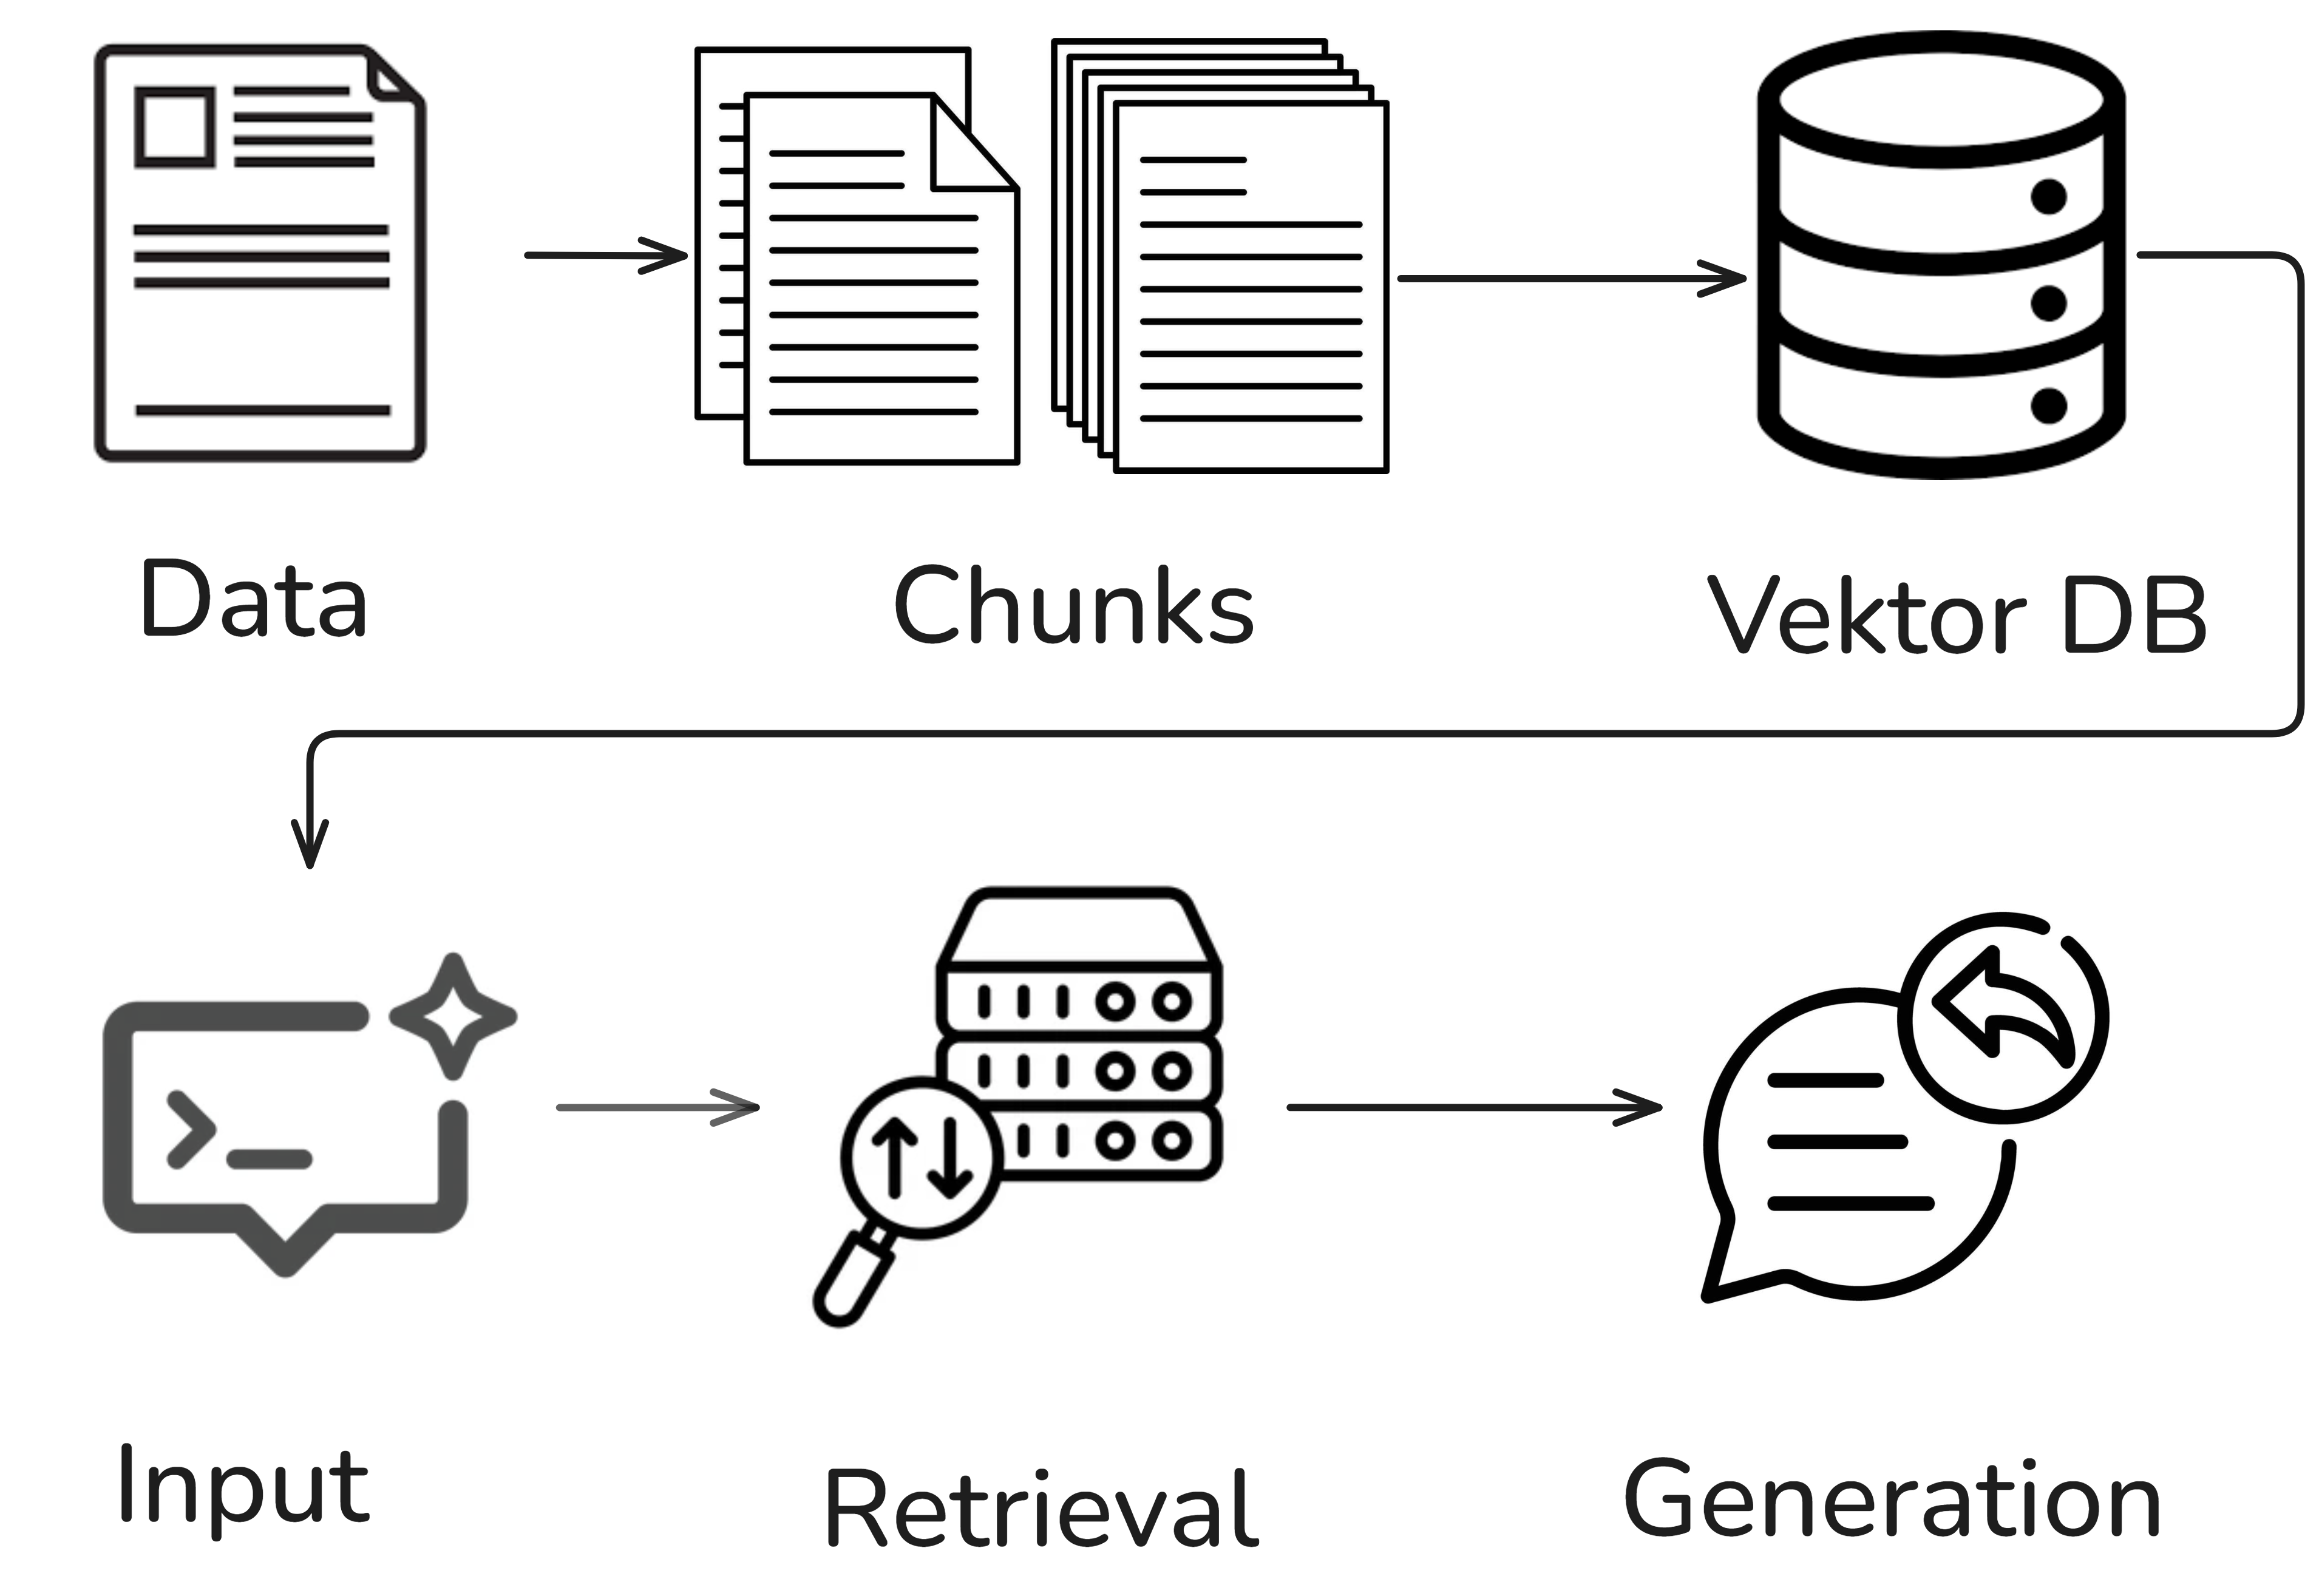
\includegraphics[width=0.9\textwidth]{image/flowrag.png}
  \caption{Alur sistem \textit{retrieval augmented generation} (RAG) saat ini}
  \label{fig:rag_as_is}
\end{figure}

Sebelum sistem RAG dapat menjawab pertanyaan, dokumen sumber terlebih dahulu melalui tahap praproses, yaitu pemotongan dokumen menjadi \textit{chunk}, pengubahan setiap \textit{chunk} menjadi representasi vektor melalui model \textit{embedding}, lalu penyimpanannya ke dalam basis data vektor (\textit{vector database}) yang menjadi sumber pengetahuan (\textit{domain knowledge}) bagi sistem. Pada domain biomedis, tahap praproses inilah yang justru banyak menimbulkan masalah. Dokumen ilmiah biomedis, khususnya abstrak pada basis data PubMed, banyak menuliskan istilah panjang dalam bentuk akronim, misalnya \textit{Hyperbaric Oxygen} yang ditulis HBO atau \textit{Coronary Heart Disease} yang ditulis CHD. Ketika \textit{chunk} yang hanya memuat akronim tersebut langsung diindeks tanpa pengayaan, representasi vektor yang terbentuk tidak memuat bentuk panjang istilahnya. Akibatnya, ketika pengguna mengajukan kueri dengan istilah lengkap, sistem \textit{retrieval} dapat gagal menemukan dokumen yang sebenarnya relevan karena terjadi ketidaksesuaian istilah antara kueri dan isi basis data vektor, fenomena yang dikenal sebagai \textit{vocabulary mismatch}. Kegagalan pada tahap \textit{retrieval} ini kemudian diteruskan ke tahap \textit{generation} dan menjadi salah satu pemicu halusinasi. Tabel~\ref{tbl:retrieval-failure} memperlihatkan beberapa contoh konkret \textit{vocabulary mismatch} tersebut.

\begin{table}[H]
\centering
\caption{Contoh \textit{Retrieval Failure} akibat \textit{Vocabulary Mismatch}}
\label{tbl:retrieval-failure}
\begin{tabular}{|p{4cm}|p{2cm}|p{6cm}|}
\hline
\textbf{Query Pengguna} & \textbf{Istilah di Paper} & \textbf{Retrieval Failure} \\ \hline
\textit{Hyperbaric Oxygen} & HBO & Gagal menemukan dokumen karena \textit{mismatch} istilah \\ \hline
\textit{Coronary Heart Disease} & CHD & Dokumen relevan tidak tertarik ke hasil \textit{retrieval} \\ \hline
\textit{Body Mass Index} & BMI & Akronim pada dokumen tidak tercocokkan dengan kueri \\ \hline
\end{tabular}
\end{table}


\subsubsection*{3.1.2 Data Understanding}

Tahap pemahaman data dilakukan untuk mengidentifikasi, menelaah, dan membandingkan himpunan data yang relevan sebagai dasar pengujian sistem berbasis \textit{retrieval augmented generation}. Fokus utama pada fase ini adalah memastikan ketersediaan data yang memiliki struktur pertanyaan yang jelas, dukungan konteks tekstual yang terikat langsung pada pertanyaan, serta tingkat kredibilitas sumber informasi yang memadai untuk dijadikan acuan evaluasi.

Sebagai langkah awal, dilakukan penelusuran terhadap dataset yang digunakan secara luas dalam penelitian model bahasa pada beberapa domain yang menuntut tingkat akurasi tinggi, yaitu hukum, kesehatan, dan keuangan. Ketiga domain dipilih karena masing-masing memiliki pola penggunaan \textit{retrieval augmented generation} yang memerlukan informasi referensial terverifikasi. Oleh sebab itu, dataset kandidat harus memuat pertanyaan terstruktur, konteks yang relevan, serta jawaban yang dapat dibandingkan secara objektif terhadap sumber informasi tertulis.

Berikut hasil pemetaan dan perbandingan dataset kandidat dari ketiga domain.

\small
\begin{longtable}{|>{\raggedright\arraybackslash}p{2.3cm}|>{\raggedright\arraybackslash}p{1.6cm}|>{\raggedright\arraybackslash}p{6cm}|>{\raggedright\arraybackslash}p{2.4cm}|}
\caption{Perbandingan Dataset Kandidat}
\label{tbl:dataset_kandidat} \\
\hline
\textbf{Nama Dataset} &
\textbf{Domain} &
\textbf{Karakteristik Utama} &
\textbf{Jumlah Data} \\
\hline
\endfirsthead

\caption[]{Perbandingan Dataset Kandidat (lanjutan)} \\
\hline
\textbf{Nama Dataset} &
\textbf{Domain} &
\textbf{Karakteristik Utama} &
\textbf{Jumlah Data} \\
\hline
\endhead

\hline
\multicolumn{4}{r}{\textit{Bersambung ke halaman berikutnya}} \\
\endfoot

\hline
\endlastfoot

CaseHOLD &
Hukum &
Pertanyaan mengenai preseden hukum berbasis putusan pengadilan federal Amerika untuk menguji kemampuan model memahami penalaran legal \parencite{casehold}. &
$\pm$ 53{,}000 contoh
\\ \hline

LegalBench &
Hukum &
Benchmark komprehensif berisi ratusan subtask untuk evaluasi penalaran hukum, interpretasi pasal, serta ekstraksi norma dan entitas legal \parencite{legalbench}. &
Variatif per subtask
\\ \hline

COLIEE &
Hukum &
Dataset berbasis kompetisi internasional untuk ekstraksi informasi dan pembuktian hubungan kasus hukum, mencakup relevansi dokumen dan ranah \textit{legal entailment} \parencite{coliee}. &
$\pm$ 4{,}000--10{,}000 contoh
\\ \hline

PubMedQA &
Kesehatan &
Pertanyaan berbasis abstrak ilmiah dalam basis PubMed dengan struktur tanya jawab faktual serta anotasi oleh pakar domain medis \parencite{pubmedqa}. &
$\pm$ 1{,}000 entri
\\ \hline

MedMCQA &
Kesehatan &
Soal pilihan ganda pendidikan kedokteran mencakup patofisiologi, diagnosis, farmakologi, dan etika klinis yang dikurasi berdasarkan silabus pendidikan medis \parencite{medmcqa}. &
$\pm$ 194{,}000 soal
\\ \hline

MMLU Medical Subset &
Kesehatan &
Subset khusus medis pada benchmark MMLU yang digunakan untuk evaluasi penguasaan konsep medis, teori klinis, anatomi, serta farmakologi \parencite{mmlu}. &
$\pm$ 80--1{,}000 pertanyaan per subkategori
\\ \hline

Financial PhraseBank &
Keuangan &
Himpunan kalimat terkait laporan keuangan perusahaan publik yang dilengkapi anotasi dan kategorisasi linguistik untuk interpretasi sentimen dan analisis ekonomi \parencite{phrasebank}. &
$\pm$ 4{,}800 kalimat
\\ \hline

Banking77 &
Keuangan &
Dataset pertanyaan layanan perbankan yang digunakan secara luas untuk pemetaan intensi pengguna serta evaluasi pemrosesan bahasa dalam layanan finansial digital \parencite{banking77}. &
$\pm$ 13{,}000 contoh
\\ \hline

\end{longtable}
\normalsize

Hasil perbandingan menunjukkan bahwa dataset pada domain hukum dan keuangan memiliki struktur data yang lebih heterogen serta melibatkan beragam bentuk pertanyaan dengan kompleksitas konteks yang tinggi. Pada dataset hukum, pertanyaan sering kali berkaitan dengan preseden yudisial, norma undang-undang, dan proses interpretasi regulasi yang memerlukan pemetaan dokumen lintas kasus. Struktur pertanyaan dan jawaban pada dataset kategori tersebut tidak selalu memiliki keterikatan langsung dengan satu konteks tunggal, sehingga dokumentasi sumber yang relevan bersifat berlapis.

Dataset pada domain keuangan memiliki karakteristik serupa. Sebagian besar himpunan data berorientasi pada interpretasi laporan, sentimen pasar, atau klasifikasi intensi pengguna dalam konteks finansial. Hubungan antara pertanyaan, sumber informasi, dan jawaban tidak selalu bersifat langsung, sehingga validasi faktualitas jawaban terhadap dokumen sumber memerlukan proses pembuktian yang lebih kompleks.

Berbeda dengan kedua domain tersebut, dataset pada ranah kesehatan menawarkan struktur data yang lebih terfokus. Konteks pertanyaan pada dataset kategori ini merujuk pada bukti ilmiah berbasis publikasi dalam jurnal kedokteran, dengan abstrak riset medis sebagai acuan utama. Salah satu dataset yang paling menonjol dibandingkan kandidat lain adalah PubMedQA.

PubMedQA memiliki karakteristik yang mendukung penerapannya pada penelitian ini. Pertama, setiap entri berisi pertanyaan yang terikat langsung dengan satu abstrak ilmiah dalam basis data PubMed. Hal ini memberikan keterhubungan yang jelas antara pertanyaan, konteks, dan jawaban, sehingga proses pembandingan kesesuaian jawaban terhadap konteks dapat dilakukan secara terukur.

Kedua, PubMedQA memiliki ukuran data yang proporsional untuk kajian akademik. Dengan total sekitar seribu entri, dataset ini representatif untuk menghasilkan analisis berbasis data tanpa memberikan beban komputasi berlebihan.

Ketiga, pertanyaan dalam PubMedQA bersifat faktual dengan format jawaban yang terstandarisasi \textit{(yes, no, dan maybe)}. Struktur tersebut mendukung pelaksanaan evaluasi berbasis kesesuaian terhadap konteks karena derajat kebenaran jawaban dapat ditelusuri secara langsung.

Keempat, PubMedQA dipilih karena karakteristik bahasanya yang sangat relevan dengan permasalahan yang diangkat pada tugas akhir ini. Abstrak paper biomedis dan kesehatan pada PubMedQA banyak menggunakan akronim atau singkatan untuk menuliskan istilah medis yang panjang, misalnya HBO untuk \textit{Hyperbaric Oxygen} atau CHD untuk \textit{Coronary Heart Disease}. Karakteristik ini menjadikan PubMedQA sebagai kasus uji yang tepat untuk menguji \textit{vocabulary mismatch}, yaitu ketidaksesuaian istilah antara kueri pengguna dan dokumen, sehingga sangat sesuai untuk mengevaluasi efektivitas ekspansi akronim sebagai salah satu teknik mitigasi yang diusulkan.

Selain itu, PubMedQA banyak digunakan dalam penelitian \textit{question answering} dan studi \textit{retrieval augmented generation} pada domain medis. Penggunaannya secara luas dalam publikasi ilmiah menjadikan dataset ini memiliki landasan metodologis yang kuat serta mempermudah pembandingan hasil penelitian dengan studi sebelumnya.

Berdasarkan keseluruhan hasil analisis pada tahap pemahaman data, PubMedQA dipandang sebagai himpunan data yang paling sesuai untuk digunakan dalam tugas akhir ini. Struktur pertanyaan yang jelas, keterikatan langsung terhadap konteks ilmiah, ukuran dataset yang proporsional, serta format jawaban yang terstandarisasi menjadikannya kandidat utama dalam proses pengujian.


\section{Analisis Kebutuhan}
\label{sec:analisis-kebutuhan}

Pada tahap ini dilakukan perumusan kebutuhan sistem yang menjadi dasar perancangan arsitektur dan eksperimen pada Tugas Akhir. Analisis kebutuhan bertujuan memastikan bahwa sistem yang dikembangkan mampu mendukung proses mitigasi halusinasi pada \textit{Retrieval-Augmented Generation} (RAG) secara terstruktur dan terukur. Kebutuhan dirumuskan berdasarkan permasalahan yang telah diidentifikasi pada analisis kondisi saat ini, mencakup kegagalan \textit{retrieval}, gangguan \textit{context noise}, dan kecenderungan model menghasilkan keluaran yang tidak \textit{faithful}. Oleh karena itu, kebutuhan sistem dibagi menjadi dua kategori utama, yaitu kebutuhan fungsional yang menggambarkan kapabilitas inti yang harus dimiliki sistem, serta kebutuhan nonfungsional yang mendefinisikan karakteristik mutu dan batasan operasional sistem. Kedua kelompok kebutuhan ini disajikan pada Tabel~\ref{tbl:kebutuhan-fungsional} dan Tabel~\ref{tbl:kebutuhan-nonfungsional}.

% ==========================================
% Tabel Kebutuhan Fungsional
% ==========================================
\begin{table}[H]
\centering
\caption{Kebutuhan Fungsional Sistem RAG-LLM untuk Mitigasi Halusinasi}
\label{tbl:kebutuhan-fungsional}
\begin{tabular}{|c|p{11cm}|}
\hline
\textbf{Kode} & \textbf{Kebutuhan Fungsional} \\ \hline

F01 & Sistem dapat menerima input berupa pertanyaan pengguna dan menghasilkan \textit{query} awal untuk proses \textit{retrieval}. \\ \hline

F02 & Sistem dapat melakukan \textit{query rewriting} untuk memperbaiki kualitas \textit{query} sebelum proses pengambilan dokumen. \\ \hline

F03 & Sistem dapat melakukan \textit{retrieval} dokumen eksternal berdasarkan \textit{query} yang telah diperbaiki. \\ \hline

F04 & Sistem dapat melakukan \textit{context reranking} untuk memilih dokumen yang paling relevan dan mengurangi \textit{context noise}. \\ \hline

F05 & Sistem dapat menghasilkan jawaban menggunakan model RAG-LLM berdasarkan konteks yang telah difilter. \\ \hline

F06 & Sistem dapat melakukan ekspansi akronim biomedis pada tahap praproses 
      dokumen untuk mengatasi \textit{vocabulary mismatch}. \\ \hline

F07 & Sistem dapat menandai atau memberi label pada segmen jawaban yang terdeteksi sebagai halusinatif. \\ \hline

F08 & Sistem dapat menghasilkan laporan evaluasi yang mencakup \textit{accuracy}, \textit{context relevancy}, \textit{context recall}, \textit{faithfulness}, \textit{F1 Score}, serta \textit{hallucination rate}. \\ \hline

F09 & Sistem dapat membandingkan keluaran dari beberapa konfigurasi eksperimen, 
      yaitu \textit{baseline}, ekspansi akronim, \textit{query rewriting}, 
      \textit{context reranking}, dan kombinasi menyeluruh. \\ \hline

\end{tabular}
\end{table}

% ==========================================
% Tabel Kebutuhan Nonfungsional
% ==========================================
\begin{table}[H]
\centering
\caption{Kebutuhan Nonfungsional Sistem RAG-LLM untuk Mitigasi Halusinasi}
\label{tbl:kebutuhan-nonfungsional}
\begin{tabular}{|c|c|p{8cm}|}
\hline
\textbf{Kode} & \textbf{Kategori} & \textbf{Kebutuhan Nonfungsional} \\ \hline

NF01 & \textit{Reliability} & Sistem harus menghasilkan proses mitigasi yang konsisten dan stabil pada berbagai set pengujian. \\ \hline

NF02 & \textit{Interpretability} & Sistem harus memberikan keluaran yang dapat ditelusuri melalui bukti serta menampilkan bagian halusinatif secara jelas. \\ \hline

NF03 & \textit{Reproducibility} & Seluruh eksperimen dapat direproduksi melalui penguncian parameter seperti \textit{temperature}, \textit{top-k}, dan \textit{max tokens}. \\ \hline

NF04 & \textit{Portability} & Sistem kompatibel dengan berbagai model LLM dan \textit{pipeline} RAG tanpa ketergantungan vendor tertentu. \\ \hline

NF05 & \textit{Ethics and Privacy} & Sistem tidak memproses data pribadi serta mengikuti prinsip \textit{responsible AI}. \\ \hline

\end{tabular}
\end{table}




\section{Analisis Pemilihan Solusi}
\label{sec:analisis-pemilihan-solusi}

\subsection{Alternatif Solusi}

Berdasarkan kajian literatur dan identifikasi kebutuhan pada sistem \textit{Retrieval-Augmented Generation (RAG)}, terdapat tiga alternatif solusi utama yang dapat diterapkan untuk mengurangi \textit{hallucination}. Setiap solusi mewakili pendekatan berbeda, baik pada tahap \textit{retrieval}, \textit{generation}, maupun \textit{post-generation}. Rincian ketiga alternatif tersebut dijelaskan sebagai berikut.

\subsubsection{Alternatif Solusi I: Penguatan Tahap \textit{Retrieval} (\textit{Query Rewriting}, \textit{Query Expansion}, dan \textit{Embedding})}

Alternatif solusi pertama berfokus pada penguatan tahap \textit{retrieval}, yaitu tahap yang menentukan kualitas konteks yang akan digunakan oleh model dalam proses generasi. Sejumlah studi menunjukkan bahwa sebagian besar \textit{hallucination} pada sistem RAG berasal dari kegagalan menemukan bukti yang benar, relevan, dan lengkap. Ketidaktepatan \textit{retrieval} menyebabkan model bekerja dengan konteks yang tidak memadai, sehingga meningkatkan peluang model mengisi kekosongan informasi dengan pengetahuan internalnya sendiri. Oleh karena itu, penguatan pada tahap \textit{retrieval} merupakan langkah fundamental dalam menurunkan risiko \textit{hallucination}.

Komponen pertama adalah \textit{query rewriting}, yaitu proses memperbaiki struktur pertanyaan pengguna sebelum proses pencarian dokumen dilakukan. Kueri asli sering kali bersifat ambigu, tidak lengkap, atau tidak mencerminkan kebutuhan informasi secara tepat. Melalui \textit{query rewriting}, pertanyaan diubah menjadi representasi yang lebih terstruktur, eksplisit, dan selaras dengan format pengetahuan dalam basis data atau korpus dokumen. Studi mutakhir menunjukkan bahwa teknik ini dapat meningkatkan presisi dokumen yang ditemukan, mengurangi \textit{retrieval error}, serta mencegah masuknya konteks yang tidak relevan yang dapat memicu \textit{hallucination}. Dengan kata lain, \textit{query rewriting} menjadi gerbang awal untuk memastikan proses pencarian bukti berjalan dengan benar.

Komponen kedua adalah \textit{query expansion}, yaitu proses memperluas cakupan kueri dengan menambahkan istilah, sinonim, atau frasa terkait yang relevan dengan maksud pertanyaan. Teknik ini bermanfaat ketika pengguna memberikan kueri yang terlalu sempit atau ketika istilah teknis tertentu memiliki banyak referensi semantik di dalam dokumen. Melalui ekspansi kueri, sistem dapat menjangkau lebih banyak kandidat dokumen yang mungkin mengandung jawaban, sehingga mengurangi risiko kehilangan bukti penting. Pendekatan ini sangat efektif pada domain dengan keragaman istilah tinggi atau pada skenario di mana pengguna tidak mengetahui terminologi yang digunakan dalam basis pengetahuan.

Komponen ketiga adalah penguatan \textit{retrieval} berbasis \textit{embedding}, yang bertujuan memetakan kueri dan dokumen ke dalam ruang vektor sehingga kesamaan semantik dapat diukur secara lebih presisi. Berbeda dengan pencarian berbasis kata kunci, metode \textit{embedding} mampu memahami kesamaan makna meskipun tidak menggunakan kata yang sama. Teknik ini memberikan dasar yang kuat dalam memilih dokumen yang relevan, terutama pada korpus besar yang mengandung variasi bahasa atau sinonim. Dengan penggunaan \textit{embedding} yang tepat, sistem dapat menemukan konteks dengan akurasi semantik yang lebih tinggi, sehingga mengurangi potensi kesalahan akibat dokumen yang tidak berhubungan.

Ketiga komponen ini bekerja saling melengkapi. \textit{Query rewriting} memastikan kueri memiliki struktur yang tepat, \textit{query expansion} memperluas cakupan pencarian agar tidak kehilangan kandidat penting, dan \textit{embedding-based retrieval} memastikan bahwa pemilihan dokumen mempertimbangkan kesamaan semantik secara lebih mendalam. Dengan demikian, risiko \textit{hallucination} dapat ditekan secara signifikan sebelum proses generasi berlangsung.


\subsubsection{Alternatif Solusi II: Penguatan Tahap \textit{Generation} melalui \textit{Middle Information}, \textit{Context Reranking}, dan \textit{Balance Internal and External Knowledge}}

Pendekatan alternatif kedua menitikberatkan pada penguatan tahap \textit{generation}, yaitu tahap ketika model membentuk jawaban akhir berdasarkan konteks yang tersedia. Meskipun informasi yang diretrieval sudah benar dan relevan, sejumlah studi menunjukkan bahwa kualitas generasi tetap dapat menurun apabila model gagal menggunakan seluruh bagian konteks secara efektif. Masalah ini terutama muncul pada skenario dengan konteks panjang, seperti pertanyaan multi-dokumen atau berlapis.

Salah satu penyebab utamanya adalah fenomena middle curse, yaitu kondisi ketika model kesulitan memanfaatkan informasi yang berada di bagian tengah konteks. Mekanisme self-attention pada arsitektur Transformer mengalami penurunan atensi terhadap token yang posisinya tidak berada di awal atau akhir, diperparah oleh keterbatasan resolusi positional encoding dan kapasitas memori ketika memproses konteks panjang. Akibatnya, meskipun informasi penting berada di bagian tengah, model sering melewatkannya sehingga akurasi generasi menurun secara signifikan. Fenomena ini tidak hanya terjadi pada tugas multi-dokumen, tetapi juga pada tugas abstraksi, penulisan jawaban panjang, dan peringkat paragraf.

Untuk mengatasi hal tersebut, teknik pemanfaatan informasi tengah (utilize the middle information) digunakan untuk menonjolkan kembali bagian konteks yang berada di tengah agar tetap terlihat oleh model selama proses generasi. Pendekatan ini dapat berupa penyesuaian bobot atensi, pengulangan segmen penting, atau penyusunan ulang konteks sehingga informasi kritis tidak tenggelam di posisi yang kurang strategis. Dengan menjamin bahwa informasi penting di bagian tengah tetap terakses, risiko kesalahan generasi yang berasal dari hilangnya bukti dapat dikurangi.

Selanjutnya, penguatan relevansi melalui \textit{context reranking} juga diperlukan pada tahap generasi. Meskipun reranking biasanya diterapkan pada tahap \textit{retrieval}, menata ulang konteks berdasarkan relevansi sebelum generasi membantu model memprioritaskan potongan informasi yang lebih penting. Hal ini sangat berguna ketika konteks berasal dari banyak dokumen atau mengandung bukti yang nilai signifikansinya berbeda. Dengan memastikan bahwa bukti paling relevan ditempatkan pada posisi yang mudah diproses model, tingkat kesalahan faktual selama generasi dapat ditekan.

Terakhir, pendekatan \textit{balancing internal and external knowledge} diperlukan untuk mengurangi kecenderungan model mengandalkan pengetahuan internalnya secara berlebihan. Pada beberapa kasus, model lebih percaya pada memorinya sendiri meskipun sudah diberikan bukti eksternal yang benar. Sebaliknya, ada kasus lain di mana model terlalu terpaku pada konteks meskipun informasi tersebut tidak lengkap. Mekanisme keseimbangan ini bertujuan menuntun model agar membandingkan dan mengonfirmasi jawaban dengan kedua sumber pengetahuan secara seimbang, sehingga hasil akhir lebih konsisten dan faktual.

Ketiga teknik ini saling melengkapi dalam memperkuat struktur pengambilan keputusan model selama tahap generasi. Dengan memastikan bahwa informasi tengah dapat dimanfaatkan, konteks relevan diprioritaskan, dan pengetahuan internal serta eksternal digunakan secara seimbang, proses generasi menjadi lebih stabil dan berbasis bukti. Hal ini berpotensi signifikan dalam menurunkan \textit{hallucination} yang muncul akibat miskonsepsi, hilangnya konteks penting, atau penggunaan bukti yang keliru.

\subsubsection{Alternatif Solusi III: \textit{Multiple-Phase Mitigation} (Ekspansi Akronim, \textit{Query Rewriting}, dan \textit{Context Reranking})}

Alternatif ketiga berfokus pada pendekatan mitigasi berlapis (\textit{multiple-phase mitigation}) yang bekerja pada beberapa tahapan dalam alur RAG, mulai dari praproses dokumen, tahap \textit{retrieval}, hingga pemilihan konteks akhir sebelum generasi. Pendekatan ini dirancang untuk mengatasi sumber utama \textit{hallucination}, yaitu kegagalan menemukan dokumen yang relevan akibat \textit{vocabulary mismatch} maupun kueri yang kurang jelas, serta masuknya konteks yang kurang relevan pada tahap generasi. Dengan menerapkan strategi mitigasi di setiap fase, sistem memperoleh perlindungan yang lebih kuat dan menyeluruh.

Komponen pertama adalah ekspansi akronim, yaitu praproses dokumen yang menyisipkan kepanjangan dari akronim biomedis secara langsung pada teks sebelum dokumen diindeks. Pada domain biomedis, banyak istilah panjang yang justru lebih sering ditulis dalam bentuk akronim pada abstrak ilmiah, sehingga kueri pengguna yang memakai istilah lengkap kerap gagal dicocokkan dengan dokumen yang relevan, fenomena yang dikenal sebagai \textit{vocabulary mismatch}. Dengan menambahkan kepanjangan akronim pada setiap dokumen, peluang pencocokan antara kueri dan dokumen meningkat, sehingga dokumen yang relevan lebih mudah ditemukan sejak tahap \textit{retrieval} dan kekosongan konteks yang memicu halusinasi dapat dikurangi.

Komponen kedua adalah \textit{query rewriting}, yaitu proses memperjelas maksud pertanyaan pengguna sebelum dokumen dicari. Tanpa perbaikan kueri, banyak sistem RAG gagal mengambil konteks yang tepat karena kueri asli pengguna sering ambigu, kurang spesifik, atau tidak mencerminkan kebutuhan informasi yang sebenarnya. Studi terkini menunjukkan bahwa kueri yang telah ditulis ulang dapat meningkatkan kualitas \textit{retrieval} secara signifikan, memperbaiki presisi dokumen yang ditemukan, serta mengurangi risiko terjadinya \textit{hallucination} yang berasal dari konteks yang kurang relevan. Dengan demikian, \textit{query rewriting} berfungsi sebagai gerbang yang memastikan proses pencarian dimulai dengan representasi pertanyaan yang paling akurat \parencite{wang2024maferw}.

Komponen ketiga adalah \textit{context reranking}, yaitu penataan ulang dokumen yang berhasil diretrieval berdasarkan tingkat relevansinya terhadap pertanyaan. Meskipun sistem berhasil menemukan sejumlah bukti yang benar, tidak semuanya memiliki nilai yang sama. Perbedaan kualitas antardokumen dapat menyebabkan \textit{context conflict} atau \textit{context noise}, di mana bukti yang kurang relevan mengaburkan bukti utama yang diperlukan model. Teknik \textit{reranking} membantu memprioritaskan dokumen dengan dukungan semantik paling kuat dan menempatkannya pada posisi yang lebih mudah diproses model selama tahap generasi. Strategi ini secara langsung mengurangi kemungkinan model menggunakan bukti yang lemah atau bertentangan, khususnya pada skenario multi-dokumen.

Ketiga teknik ini membentuk alur mitigasi bertahap yang saling melengkapi. Ekspansi akronim memperbaiki keterjangkauan dokumen sejak tahap praproses dan pengindeksan, \textit{query rewriting} mencegah kesalahan pada tahap pencarian bukti, dan \textit{context reranking} memastikan hanya bukti terbaik yang menjadi dasar generasi. Dengan perlindungan berlapis pada tahap praproses, \textit{retrieval}, dan pemilihan konteks, risiko kesalahan dapat ditekan dari hulu hingga hilir, menghasilkan sistem RAG yang lebih akurat, lebih dapat dipercaya, dan lebih tahan terhadap variasi pertanyaan serta kompleksitas konteks.



\subsection{Analisis Penentuan Solusi}
\label{subsec:analisis-penentuan-solusi}

Setelah merumuskan beberapa alternatif solusi mitigasi \textit{hallucination} pada sistem \textit{Retrieval-Augmented Generation (RAG)}, langkah berikutnya adalah menentukan solusi yang paling tepat untuk diterapkan dalam tugas akhir ini. Penentuan solusi dilakukan menggunakan pendekatan \textit{weighted scoring}, yaitu metode evaluasi alternatif berdasarkan sejumlah kriteria yang diberi bobot sesuai tingkat kepentingannya. Setiap alternatif diberi skor menggunakan skala \textit{Likert} satu sampai sepuluh untuk masing-masing kriteria, kemudian dihitung skor total tertimbangnya.

Empat kriteria utama yang digunakan adalah sebagai berikut.  

\textbf{Efektivitas} menilai sejauh mana suatu alternatif mampu mengurangi \textit{hallucination} pada sistem RAG–LLM. Kriteria ini menjadi prioritas utama karena \textit{hallucination} berdampak langsung pada keakuratan informasi dan kepercayaan pengguna. Tugas Akhir terdahulu menunjukkan bahwa kesalahan faktual, termasuk misinformasi dalam domain sensitif seperti kesehatan, hukum, dan keuangan, dapat menimbulkan konsekuensi serius bagi individu maupun institusi \parencite{pang2024medical}. Oleh karena itu, alternatif dengan skor efektivitas tinggi diharapkan mampu menurunkan \textit{intrinsic hallucination} dan \textit{factual hallucination} secara signifikan.

\textbf{Feasibility} mengukur sejauh mana alternatif solusi realistis untuk diimplementasikan dalam konteks Tugas Akhir ini, baik dari segi kompleksitas teknis, ketergantungan terhadap infrastruktur, maupun ketersediaan alat dan \textit{library}. Solusi dengan feasibility tinggi bersifat masuk akal untuk diwujudkan pada lingkungan eksperimen dengan sumber daya terbatas, tanpa mengorbankan kualitas mitigasi \textit{hallucination}.

\textbf{Biaya komputasi} mengevaluasi kebutuhan sumber daya yang diperlukan masing-masing alternatif, misalnya jumlah pemanggilan \textit{API}, beban \textit{retrieval}, beban \textit{reranking}, serta operasi tambahan seperti verifikasi berulang atau generasi multipel. Semakin tinggi skor pada kriteria ini berarti alternatif solusi menggunakan sumber daya yang relatif lebih hemat dan efisien untuk dijalankan pada skala eksperimen yang luas.

\textbf{Fleksibilitas} menilai kemampuan alternatif solusi untuk dikembangkan, diadaptasi, atau diperluas di masa depan. Solusi yang fleksibel cenderung bersifat modular, tidak terlalu terikat pada satu jenis LLM atau satu skenario tugas, serta mudah diintegrasikan dengan teknik mitigasi tambahan yang mungkin dikaji pada tugas akhir lanjutan.

Tiga alternatif solusi yang dibandingkan dalam tugas akhir ini adalah:
\begin{enumerate}[1.]
  \item \textbf{Solusi I: Penguatan \textit{retrieval}} (\textit{query rewriting} + \textit{query expansion} + \textit{context reranking}), yang berfokus pada peningkatan kualitas kueri dan seleksi konteks sejak tahap pengambilan informasi.
  \item \textbf{Solusi II: Penguatan \textit{generation}} (\textit{faithfulness prompting} + \textit{attribution prompting} + \textit{chain-of-verification}), yang mengandalkan desain \textit{prompt} dan verifikasi berjenjang untuk menjaga kesetiaan jawaban terhadap konteks.
  \item \textbf{Solusi III: Solusi tugas akhir} (ekspansi akronim + \textit{query rewriting} + \textit{context reranking}), yang menggabungkan praproses ekspansi akronim untuk mengatasi \textit{vocabulary mismatch}, perbaikan kueri sebelum \textit{retrieval}, serta pemilihan konteks paling relevan sebelum generasi.
\end{enumerate}

Bobot kriteria yang digunakan dalam skema \textit{weighted scoring} ditetapkan sebagai berikut: efektivitas sebesar 40\%, feasibility sebesar 25\%, biaya komputasi sebesar 20\%, dan fleksibilitas sebesar 15\%. Bobot ini ditentukan berdasarkan prioritas penelitian terhadap efektivitas mitigasi halusinasi sebagai sasaran utama, diikuti kompleksitas implementasi dan efisiensi komputasi sebagai pertimbangan praktis. Skor untuk masing-masing alternatif kemudian dihitung dengan mengalikan skor \textit{Likert} dengan bobot kriteria terkait, lalu menjumlahkannya menjadi skor total tertimbang. Ringkasan hasil penilaian disajikan pada Tabel~\ref{tbl:weighted_scoring_solusi}.

\begin{table}[H]
  \centering
  \caption{Kalkulasi \textit{weighted scoring} pada alternatif solusi mitigasi \textit{hallucination}}
  \label{tbl:weighted_scoring_solusi}
  \begin{tabular}{|p{3cm}|c|c|c|c|}
    \hline
    \multicolumn{1}{|c|}{\textbf{Kriteria}} &
    \textbf{Bobot} &
    \multicolumn{3}{c|}{\textbf{Alternatif Solusi}} \\
    \cline{3-5}
    & &
    \textbf{Solusi I} &
    \textbf{Solusi II} &
    \textbf{Solusi III} \\
    \hline

    Efektivitas & 40\% &
    8 & 7 & 9 \\
    \hline

    \textit{Feasibility} & 25\% &
    7 & 6 & 9 \\
    \hline

    Biaya komputasi & 20\% &
    7 & 5 & 7 \\
    \hline

    Fleksibilitas & 15\% &
    8 & 7 & 8 \\
    \hline

    \multicolumn{2}{|c|}{\textbf{Skor total}} &
    \textbf{7,55} &
    \textbf{6,35} &
    \textbf{8,45} \\
    \hline
  \end{tabular}
\end{table}



Berdasarkan hasil \textit{weighted scoring} pada Tabel~\ref{tbl:weighted_scoring_solusi}, Solusi III memperoleh skor total tertinggi (8,45) dibandingkan dua alternatif lainnya. Hal ini mencerminkan kombinasi yang seimbang antara efektivitas pengurangan \textit{hallucination}, feasibility implementasi yang tinggi karena ekspansi akronim merupakan praproses sederhana, biaya komputasi yang hemat karena tidak menambah pemanggilan model pada saat \textit{inference}, serta fleksibilitas untuk dikembangkan lebih lanjut. Oleh karena itu, tugas akhir ini memilih Solusi III, yaitu kombinasi ekspansi akronim, \textit{query rewriting}, dan \textit{context reranking}, sebagai pendekatan utama mitigasi \textit{hallucination} pada sistem RAG-LLM.

Selain hasil \textit{weighted scoring}, pemilihan Solusi III juga didukung oleh temuan penelitian yang menunjukkan bahwa penggabungan beberapa teknik mitigasi dalam satu alur kerja dapat meningkatkan performa RAG–LLM secara nyata. Salah satu pendekatan adalah RAG-HAT (\textit{RAG–Hallucination-Aware Tuning}), yang mengintegrasikan deteksi \textit{hallucination}, perbaikan jawaban, dan penyesuaian model melalui \textit{preference optimization}. Penelitian ini melaporkan penurunan \textit{hallucination} hingga 27-44\% dibandingkan RAG standar \parencite{song2024raghat}, menunjukkan bahwa pendekatan multi-tahap efektif meningkatkan performa RAG.

Pendekatan lain yang relevan adalah MEGA-RAG, yang menggabungkan \textit{dense retrieval}, \textit{cross-encoder reranking}, dan penggabungan bukti sebelum proses generasi. Hasilnya, akurasi sistem meningkat sekitar 8-14\% pada berbagai tugas \textit{knowledge-intensive QA} dibandingkan RAG tanpa mekanisme gabungan \parencite{li2023megarag}. Temuan ini memperlihatkan bahwa penggabungan teknik memberikan dampak langsung pada peningkatan kualitas jawaban.

Berdasarkan kedua studi tersebut, terlihat jelas bahwa pendekatan yang menggabungkan beberapa teknik mitigasi pada tahap praproses, \textit{retrieval}, dan pemilihan konteks lebih mampu meningkatkan akurasi dan mengurangi \textit{hallucination} secara konsisten. Oleh karena itu, pemilihan Solusi III dalam tugas akhir ini memiliki landasan yang kuat, karena menggabungkan ekspansi akronim, \textit{query rewriting}, dan \textit{context reranking} yang sejalan dengan arah penelitian terbaru.